\documentclass[10pt,a4paper]{article}
\usepackage[latin1]{inputenc}
\usepackage{amsmath}
\usepackage{amsfonts}
\usepackage{amssymb}
\usepackage{graphicx}
\usepackage{float}
\author{Michele De Vita}
\begin{document}
	\begin{enumerate}
		\item  
		\begin{align*}
	 &i) \,\,\, \mathbf{C} = (0,  5, -7, 0), &d = -2  \\
		& ii) \,\,\, \mathbf{C} = (0, 2, -1, -1, 0),  &d=0 
		\end{align*}
		\item 
		This plot shows the SSE in function of $ \beta $:
		\begin{figure}[H]
			\centering
			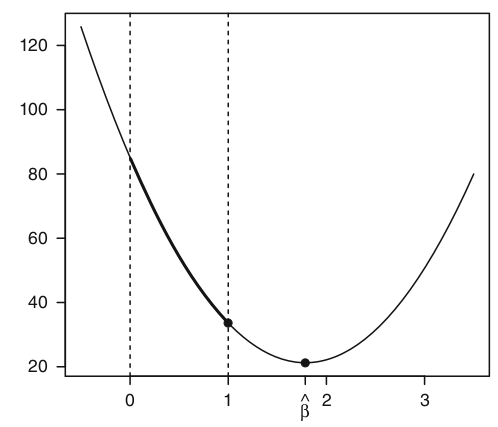
\includegraphics[width=0.7\linewidth]{plot_ftest}
		\end{figure}
		The F-test score is $ \dfrac{SSE_{H_0} - SSE}{SSE} $ where $ SSE = SSE(\hat{\beta}) $ that is the y in the plot where $ x = \hat{\beta} $ and $ SSE_{H_0} = SSE(\beta = 1) $\\
		The plot for the numerator of Wald test is the same of the previous because the numerator is the same except for a square difference instead of normal difference.\\
		The main difference between F-test and Wald test is the denominator in the first is $ \hat{\theta} $ while in the second is $ var(\hat{\theta}) $. There is also a relation between test statistics $ F $ and $ W $: $ W = rF $
		\item The confidence interval for $ \mu_0  $ is $ \mathbf{x}_0' \hat{\beta} \pm t_{n-p}(1-\alpha / 2) \hat{\sigma} (\mathbf{x}_0' (\mathbf{X'X})^{-1} x_0)^{1/2}$ while for prediction is $ \mathbf{x}_0' \hat{\beta} \pm t_{n-p}(1-\alpha / 2) \hat{\sigma} (1 + \mathbf{x}_0' (\mathbf{X'X})^{-1} x_0)^{1/2}$. The difference between the two formulas is the "$ 1\,\,+ $" near $ x_0 $ that become from the fact that the estimation try to give an confidence interval of a parameter , so with no variance, while the prediction try to estimate a aleatory variable with a expected value and a variance.
		\item $ f(x_0) = \mathbf{x}_0' \hat{\beta} \pm t_{n-2}(1-\alpha / 2) \hat{\sigma} (1 + \mathbf{x}_0' (\mathbf{X'X})^{-1} x_0)^{1/2}$
		where $ X = $
		$ \left( \begin{matrix}
			1 & x_{11} \\ 
			\vdots & \vdots  \\ 
		1 & x_{n1}
			\end{matrix} \right)$ and $ p = 2 $.\\
			The length of interval is minimum when $ \mathbf{x_0 = 0}  $
			\item Increasing the number of parameters is not always a good idea: we can express the SPSE (expected squared prediction error as):
			$ \underbrace{n\sigma^2}_{irreducible\,\,  part} + \underbrace{|M|\sigma^2}_{Variance \,\, error} + \underbrace{\sum_{i=1}^{n} (u_{i M} - u_i)^2}_{BIAS^2} $
			\item If we consider only $ \mathbf{X_1} $ we have $ \mathbf{X = X_1} $ then 
			\begin{align*}
				E\left[ \tilde{\beta}_1 \right]		&= E \left[ \mathbf{(X_1'X_1)^{-1} X_1'y} \right] \\
				&=  \mathbf{(X_1'X_1)^{-1} X_1' } E \left[ \mathbf{y} \right] \\
				&=  \mathbf{(X_1'X_1)^{-1} X_1' (X_1 \beta_1 + X_2 \beta_2)} \\
				&= \beta_1 +\mathbf{(X_1'X_1)^{-1} X_1'  X_2 \beta_2}
			\end{align*}
			The bias vanish if $ \mathbf{X_1'  X_2  = 0} $ that in statical words mean that $ \mathbf{X_1} \text{ and } \mathbf{X_2} $ are uncorrelated 
	\end{enumerate}
\end{document}